\documentclass[12pt,]{article}
\usepackage[left=1in,top=1in,right=1in,bottom=1in]{geometry}
\newcommand*{\authorfont}{\fontfamily{phv}\selectfont}
\usepackage[]{mathpazo}


  \usepackage[T1]{fontenc}
  \usepackage[utf8]{inputenc}




\usepackage{abstract}
\renewcommand{\abstractname}{}    % clear the title
\renewcommand{\absnamepos}{empty} % originally center

\renewenvironment{abstract}
 {{%
    \setlength{\leftmargin}{0mm}
    \setlength{\rightmargin}{\leftmargin}%
  }%
  \relax}
 {\endlist}

\makeatletter
\def\@maketitle{%
  \newpage
%  \null
%  \vskip 2em%
%  \begin{center}%
  \let \footnote \thanks
    {\fontsize{18}{20}\selectfont\raggedright  \setlength{\parindent}{0pt} \@title \par}%
}
%\fi
\makeatother




\setcounter{secnumdepth}{0}

\usepackage{longtable,booktabs}



\title{Social Capital and the Success of Economic
Sanctions \thanks{\textbf{Current version}: Feburary/02/2021;
\textbf{Corresponding Author}: Taehee Whang
(\href{mailto:thwhang@yonsei.ac.kr}{\nolinkurl{thwhang@yonsei.ac.kr}})}  }
 



\author{\Large Jaeyoung Hur\vspace{0.05in} \newline\normalsize\emph{The
Global Leaders College, Yonsei University}   \and \Large Sanghoon
Park\vspace{0.05in} \newline\normalsize\emph{Department of Political
Science}   \and \Large Hannah
Kim\vspace{0.05in} \newline\normalsize\emph{Department of Political
Science, University of Nebraska, Omaha}   \and \Large Taehee
Whang\vspace{0.05in} \newline\normalsize\emph{Department of Political
Science and International Studies, Yonsei University}  }


\date{}

\usepackage{titlesec}

\titleformat*{\section}{\normalsize\bfseries}
\titleformat*{\subsection}{\normalsize\itshape}
\titleformat*{\subsubsection}{\normalsize\itshape}
\titleformat*{\paragraph}{\normalsize\itshape}
\titleformat*{\subparagraph}{\normalsize\itshape}


\usepackage{natbib}
\bibliographystyle{apsr}
\usepackage[strings]{underscore} % protect underscores in most circumstances



\newtheorem{hypothesis}{Hypothesis}
\usepackage{setspace}


% set default figure placement to htbp
\makeatletter
\def\fps@figure{htbp}
\makeatother

\usepackage{hyperref}
\usepackage{ntheorem}\theoremseparator{:}
\newtheorem{hyp}{Hypothesis}
\usepackage{graphicx}
\usepackage{caption, threeparttable}
\usepackage{booktabs}
\usepackage{longtable}
\usepackage{array}
\usepackage{multirow}
\usepackage{wrapfig}
\usepackage{float}
\usepackage{colortbl}
\usepackage{pdflscape}
\usepackage{tabu}
\usepackage{threeparttable}
\usepackage{threeparttablex}
\usepackage[normalem]{ulem}
\usepackage{makecell}
\usepackage{xcolor}

% move the hyperref stuff down here, after header-includes, to allow for - \usepackage{hyperref}

\makeatletter
\@ifpackageloaded{hyperref}{}{%
\ifxetex
  \PassOptionsToPackage{hyphens}{url}\usepackage[setpagesize=false, % page size defined by xetex
              unicode=false, % unicode breaks when used with xetex
              xetex]{hyperref}
\else
  \PassOptionsToPackage{hyphens}{url}\usepackage[draft,unicode=true]{hyperref}
\fi
}

\@ifpackageloaded{color}{
    \PassOptionsToPackage{usenames,dvipsnames}{color}
}{%
    \usepackage[usenames,dvipsnames]{color}
}
\makeatother
\hypersetup{breaklinks=true,
            bookmarks=true,
            pdfauthor={Jaeyoung Hur (The Global Leaders College, Yonsei
University) and Sanghoon Park (Department of Political
Science) and Hannah Kim (Department of Political Science, University of
Nebraska, Omaha) and Taehee Whang (Department of Political Science and
International Studies, Yonsei University)},
             pdfkeywords = {Economic sanctions, social capital, North
Korea, opposition effect, rally effect},  
            pdftitle={Social Capital and the Success of Economic
Sanctions},
            colorlinks=true,
            citecolor=blue,
            urlcolor=blue,
            linkcolor=magenta,
            pdfborder={0 0 0}}
\urlstyle{same}  % don't use monospace font for urls

% Add an option for endnotes. -----


% add tightlist ----------
\providecommand{\tightlist}{%
\setlength{\itemsep}{0pt}\setlength{\parskip}{0pt}}

% add some other packages ----------

% \usepackage{multicol}
% This should regulate where figures float
% See: https://tex.stackexchange.com/questions/2275/keeping-tables-figures-close-to-where-they-are-mentioned
\usepackage[section]{placeins}


\begin{document}
	
% \pagenumbering{arabic}% resets `page` counter to 1 
%    

% \maketitle

{% \usefont{T1}{pnc}{m}{n}
\setlength{\parindent}{0pt}
\thispagestyle{plain}
{\fontsize{18}{20}\selectfont\raggedright 
\maketitle  % title \par  

}

{
   \vskip 13.5pt\relax \normalsize\fontsize{11}{12} 
\textbf{\authorfont Jaeyoung Hur} \hskip 15pt \emph{\small The Global
Leaders College, Yonsei University}   \par \textbf{\authorfont Sanghoon
Park} \hskip 15pt \emph{\small Department of Political
Science}   \par \textbf{\authorfont Hannah
Kim} \hskip 15pt \emph{\small Department of Political Science,
University of Nebraska, Omaha}   \par \textbf{\authorfont Taehee
Whang} \hskip 15pt \emph{\small Department of Political Science and
International Studies, Yonsei University}   

}

}








\begin{abstract}

    \hbox{\vrule height .2pt width 39.14pc}

    \vskip 8.5pt % \small 

\noindent What determines the success of economic sanctions? Although
numerous studies explore the formal institutional characteristics of
sanctioned countries and their effects on sanction effectiveness, few
examine informal social institutions such as trust, membership, or, more
broadly, social capital. Using the latest Threat and Imposition of
Economic Sanctions data and cross-national World Values Survey data,
this study examines how trust and social capital in sanctioned countries
affect the target governments' ability to endure the costs of economic
sanctions. The findings support our theory that sanctions are less
likely to be effective when imposed on countries with high trust,
membership, and confidence in political institutions.


\vskip 8.5pt \noindent \emph{Keywords}: Economic sanctions, social
capital, North Korea, opposition effect, rally effect \par

    \hbox{\vrule height .2pt width 39.14pc}



\end{abstract}


\vskip -8.5pt


 % removetitleabstract

\noindent \doublespacing 

\hypertarget{introduction}{%
\section{Introduction}\label{introduction}}

When North Korea conducted its first underground nuclear test in 2006,
the United Nations (U.N.) adopted resolution 1718, acting unanimously
under Chapter VII of the UN Charter. With six nuclear tests between
October 2006 and September 2017, the economic sanctions have been
strengthened every time. The initial sanctions targeted Kim Jong-il and
his supporters for the nuclear weapons program by restricting their
ability to travel, prohibiting the flow of luxurious goods, and freezing
their financial accounts abroad.\footnote{The recent United Nations
  Security Council (UNSC) Resolution 2375 included contents such as a
  Maritime Interdiction of Cargo Vessels, a limit to the import of crude
  oil, textile, fully completed apparel and coal, as well as a
  prohibition of exports and joint ventures. By comparing the UNSC
  Resolution 1718, which was passed after the first nuclear test and the
  UNSC Resolution 2375, which was passed after the 6th nuclear test, we
  can clearly see that the range and degree of the economic sanctions
  have been strengthened.}

These targeted sanctions have not curbed Pyongyang's nuclear ambitions.
Policymakers in South Korea have been discussing ways to increase the
effectiveness of these sanctions since North Korea's nuclear tests on 6
January 2016 and 9 September 2016. The South Korean Ministry of
Unification announced one such effort---closing the Kaesong industrial
complex---in February 2016. This action was part of a general strategy
to increase the number of North Koreans afflicted by sanctions in the
hope of inciting the populace to force Kim Jong-un to amend his
policies.\footnote{In May 2017, the South Korean government acted upon
  the appeasement of North Korea and held three Inter-Korean Summit
  meetings, however, there seems to be no visible progress on the
  lifting of economic sanctions yet. Furthermore, the U.S.-DPRK Summits
  in June 2018 and February 2019 both fail to show fundamental change in
  the sanctions towards North Korea.}

When a sender imposes a sanction, it can be expected that it will damage
the targeted states' economies and increase the political and economic
costs of a leader in the targeted states. Therefore, for an economic
sanction to be successful, it is essential that a sanction is costly for
the leader. However, sanctions sometimes are not costly. For instance,
when North Korea confronted economic sanctions, its leader declared that
he regards sanctions as an act of war \citep{frank2006a}. Then, citizens
are most likely or mobilized to support the leadership in the face of
foreign coercion \citep{cortright2002a}.

Therefore, this leads to the question, whether and under what
circumstances economic sanctions succeed? Firstly, it is plausible that
shifting the burden of sanctions might rouse the general populace to
confront its government and force a policy change, particularly if the
sanctions were imposed for reasons seemingly unrelated to ordinary
citizens. In other words, a populace can be mobilized from the bottom up
if people believe they are being afflicted by a kind of tariff imposed
only because its leaders behave in a certain way. Plausibility
notwithstanding, however, we argue that one important construct can
prevent this strategy from succeeding: social capital.

Social capital embodies collective values such as trust, membership, and
confidence in institutions that unite people. When assessing sanctions,
social capital matters as the success of the sanctions may depend on the
likelihood of mobilizing an afflicted populace from the bottom. When the
nature of a nation's social capital is such that it can unite a populace
to demand policy changes from its leader, we posit that an
\emph{opposition effect} favors the success of the sanctions. When the
nature of social capital is such that it unites the populace behind a
leader who defies the sanctions, we posit that a \emph{rally effect}
assures that more comprehensive sanctions will fail.

Drawing from two datasets spanning 1981 to 2005---the Threat and
Imposition of Sanctions (TIES) and the World Values Survey (WVS)---we
investigate whether the \emph{opposition effect} or the \emph{rally
effect} of social capital dominates a populace's response to sanctions.
We empirically demonstrate which of the two contradictory effects can be
observed using the data. If social capitals have opposite effects on
economic sanctions, a populace is likely to mobilize effectively against
their leader to let him comply with the sanctions. Otherwise, a
sanctioned country's populace shares high degrees of interpersonal
trust, membership in social or political organizations, confidence in
key institutions, and they support the leader to fight against economic
sanctions.

This paper proceeds as follows. The second section studies literature
related to social capital, and the third explains the theoretical
effects of social capital in response to sanctions. The fourth section
describes the data collection, variables, and methods. The fifth
presents the empirical findings, and the sixth section concludes.

\hypertarget{literature-reviews}{%
\section{Literature Reviews}\label{literature-reviews}}

\hypertarget{social-captial}{%
\subsection{Social captial}\label{social-captial}}

\citet{putnam1993a} and \citet{putnam2000a} introduced the concept of
social capital as `features of social organizations such as networks,
norms, and social trust that facilitate coordination and cooperation for
mutual benefit' \citep[65]{putnam2000a}. Social capital remains
much-discussed in political science and is particularly used to explain
phenomena such as political participation. The origins of social capital
appear in the works of \citet{bourdieu1986a} and \citet{coleman1988a},
and the concept continues to be defined generally as degrees of trust,
networks built through association (membership), and the confidence
people feel within their communities.

\citet{bourdieu1986a} perceived social capital as the
institutionalization of relationships and mutual acquaintance and the
sum of the benefits or opportunities that an individual or an
institution will achieve, both real or virtual, through a network.
\citet{coleman1988a} defined social capital as an aspect of social
relations or social structure in which certain actions become possible
for an individual through participation. In addition, \citet{brehm1997a}
viewed social capital as a similar concept to a cooperative network
(social network) within the community where individuals' engagement in
communities created higher levels of interpersonal trust and thus,
promoted collective action between citizens to facilitate the resolution
of problems within that community.

High degrees of social capital enhance societies and their effective
functioning. Three of its aspects are particularly influential and can
be measured. The first is trust, which heightens a sense of inclusion.
As trust increases, members are more likely to support and protect the
community. The second is membership, which allows for smaller groups of
like-minded people to create dense networks that engender information
flow. Finally, confidence is about high levels of social capital
developed within communities. When the populace has confidence in their
communities, they tend to show greater political efficacy.

Empirical studies generally employ social capital as a dependent
variable. However, prominent scholars use it as an explanatory variable
to explain democratic or economic performance
\citep[\citet{fukuyama1995a}]{putnam1993a}. The \emph{critical citizen
theory} and \emph{dissatisfied democrat theory}, for example, contend
that political participation increases when people are dissatisfied
within their communities \citep{dalton2015a}. \citet{a1963a}, \emph{The
Civic Culture}, clarifies how feelings of efficacy inspire confidence
among the populace and encourage people to contribute to their
societies. Through feelings of efficacy, political participation
increases as trust and confidence increase within a community.

Research into social capital mainly addresses comparative politics, and
extensive survey research compares and contrasts degrees of social
capital in countries and regions. By observing social capital within the
framework of international relations and particularly the international
political economy, we observe how social capital contributes to
resisting sanctions. In measuring social capital, according to degrees
of intra-community trust, membership, and confidence, we theorize
whether higher degrees of social capital encourage a populace to defy
sanctions and resist policy concessions.

\hypertarget{economic-sanctions}{%
\subsection{Economic Sanctions}\label{economic-sanctions}}

Traditionally, scholars considered economic sanctions as a substitute
for military intervention, defining the concept as the tools of economic
statecrafts to achieve only political goals, not economic goals
\citep{pape1997a}. However, it is challenging to distinguish economic
sanctions between political goals and other types of goals. Thus,
another line of studies attempts to expand its concept, suggesting that
economic sanction should be more than just economic coercion for
political goals. For example, \citet{baldwin1985a} states that economic
sanctions are statecrafts that reveal a strong willingness to audiences
in third countries and pursue changes more than target states'
attitudes.

As the concept of economic sanctions extends beyond various types of
goals, it implies `deliberate, government-inspired withdrawal, or threat
of withdrawal, of customary trade or financial relations' to `achieve
foreign policy goals' \citep{hufbauer2007a}, or the limitations or
disconnections of economic relations, which are aimed at changing the
relevant policies of the countries in dispute \citep{morgan2009a}. In
sum, economic sanctions scholarships have a consensus on an instrumental
definition that economic sanctions should include economic mechanisms,
but the outcomes are not restricted to the economic area.

Conventional wisdom insists that sanctions do not provoke meaningful
compliance from the sanctioned country. As \citet{hufbauer2007a} note,
sanctions `may simply be inadequate for the task. The goals may be too
elusive; the means too gentle; or cooperation from other countries, when
they needed, too tepid'. In a little over 25\% of the cases they
examined, sanctions exerted costs estimated to exceed 2\% of sanction
nations' GNP. Altogether, sanctions do not seem always to impose severe
economic consequences.

Given the general ineffectiveness of sanctions, scholars pose two
questions: `Why do policymakers still impose them?' and `What
conditions, if any, might be conducive to successful sanctions?' We seek
to answer the latter question by observing degrees of social capital in
sanctioned countries. We posit that social capitals--trust, membership,
and confidence in institutions--are significant in determining whether a
populace supports or resists its leader's response to sanctions.

\hypertarget{theory}{%
\section{Theory}\label{theory}}

\hypertarget{economic-sanctions-and-social-capitals}{%
\subsection{Economic sanctions and social
capitals}\label{economic-sanctions-and-social-capitals}}

Let us assume that country A, i.e., sender, and country B, i.e., target,
are in a trade dispute and country A decides to impose sanctions that
inflict sufficient economic hardships on country B to cause it to alter
its policy. Country B suffers direct hardships via economic losses
(reduced trade, investment, or GDP) and indirect hardships via burdens
on its populace. Such burdens might include less government spending on
public health \citep{marks1999a}, reduced disaster prevention and
mitigation \citep{mclean2019a}, and fewer anti-terrorism initiatives
\citep{navin2016a}. Country B's leader can defy A's sanctions and uphold
existing policies or make partial or comprehensive concessions to A's
demands.

Although earlier literature treats countries A and B as unitary actors
\citep{lacy2004a}, this study departs from these dyadic assumptions by
modeling whether social capital influences the extent to which the
leader of the country B can defy the sanctions. In this study we posit
that social capital influences how the populace might react, which
affects the leader of country B's decision via two mechanisms that let
the populace mobilize against their leader, or rally around their leader
against the sanction; and this study in we use the customary approach.
Numerous studies analyze the role of within-state actors or domestic
institutions in determining sanctions or threats. However, most studies
focus on domestic political institutions within the sanction-imposing
country \citep{cox2006a}, among interest groups \citep{kaempfer1992a},
and with voters \citep{mcgillivray2004a} and few studies examine the
internal and social characteristics of the sanctioned countries. Several
studies document how rally-round-the-flag effects lead to failed
sanctions in the targeted states \citep{allen2005a, allen2008a},
however, few systematize the conditions under which these effects work
successfully. We find that the degree of social capital in the
sanctioned country illuminates the issue, although it can lead to
potentially contradictory results.

Assuming sanctions are in place, we argue that social capital measured
by the dimensions of trust, membership, and confidence in political
institutions affects how the leaders of sanctioned countries react to
sanctions. In this study we develop how social capital can generate
\emph{opposition effects} and \emph{rally effects} among the populace of
sanctioned countries and demonstrate that they potentially influence
whether sanctions succeed.

\hypertarget{opposition-effect}{%
\subsection{Opposition effect}\label{opposition-effect}}

Traditional explanations of economic sanctions focus on punishment,
stating that the more painful the sanctions, the greater is the
possibility of the target state facing political disintegration. It
implies that when sanctions negatively affect the standard of living in
a target state, these social hardships provide the ruled populace in the
targeted states the incentives to mobilize and pressurize the government
to comply with the senders' demands \citep[850]{lektzian2007a}. It is
challenging that sanctions are always `smart', which means that even
targeted sanctions on specific groups within the targeted states can
affect all domestic actors in the target. For example, on 7 August 2018,
the Trump administration in the US completely restored UN sanctions
against Iran. The sanctions against Iran date back to the time of the
Iranian Revolution in 1979. The US argues that the sanctions against
Iran target the Iranian government, not Iranian citizens. Nevertheless,
the US economic sanctions severely harm the everyday lives of Iranian
citizens. The sanctions restricted the Iranian citizens' access to daily
necessities due to rising prices. Medicine was one of the typical
necessities that Iranian citizens faced challenges to procure. Although
the US sanctions do not directly restrict the medicine supply chain,
medicine companies refuse to sell their product in Iran, taking into
account their relationship with the United States. Consequently,
patients who have cancer, epilepsy, and hemophilia have difficulties in
treatment. Even if Iran tries to produce substitutes domestically, it is
difficult to obtain essential ingredients due to sanctions
\citep{bbc2014}.

From the perspective of the targeted state's society, sanctions are a
tariff, even if they are imposed for reasons unrelated to trade, such as
in response to the development of weapons of mass destruction and it is
reasonable to expect the targeted society will hold its leader
accountable for policies that generate these sanctions.

In this study we maintain that social capital supplements the gaps in
the theoretical arguments concerning winning coalitions, encouraging
people to collaborate and mobilize to demand policy concessions from
their leader. Facing the mobilization, the leader should feel the
pressure when he keeps fighting against economic sanctions. In other
words, such mobilization provides an opposition effect, which makes the
leader more likely to reverse his policies and comply with sanctions.
Sanctions are more likely to be successful when social capital is higher
as the increased social capital enables more effective collective
action. This study develops the following hypothesis from this argument:
\newline

\begin{hyp}\label{opposition} {\bf Opposition Effect}: As the level of social capital increases, the likelihood of sanction success increases.\end{hyp}

\hypertarget{rally-effect}{%
\subsection{Rally effect}\label{rally-effect}}

In this opposing scenario, strong internal ties in the sanctioned
country prompt the populace to rally around its leaders. As with the
\emph{opposition effect}, the public bears most of the onus of sanctions
and does not criticize the government's policy because social capital
creates conditions that support the leader's decision to defy sanctions.
For many cases of sanctions, it is also possible that social capital
creates an environment in which the leader can employ social capital for
personal political purposes. The leader dominates resources, controls
information, and blames outside intervention by framing the sanctioned
country as a victim of international conflicts.\footnote{Note that there
  are many sanctioned countries that are led by a strongman who dictates
  the conditions under which social capital is formed.} The populace
consequently views sanctions as foreign interference and finds no need
to revolt against them. The leader thus has an incentive to use high
social capital as a tool to create a \emph{rally effect} through which
people are inspired to support resistance to sanctions and the
sanctioned government continues its controversial policy. High degrees
of social capital in a sanctioned country can be a double-edged sword in
this regard.

In sum, there are two reinforcing effects that lead to the condition
that is favorable to the leader of the sanctioned country. While social
capital can spontaneously generate support to an extent, the leader can
also manipulate the sources of information that create support. Thus,
there are two kinds of \emph{rally effects}--one spontaneous and another
contrived. In reality, it is not easy to differentiate between the
actions that create social capital, appeal to social capital, and
suppress the \emph{opposition effect}. However, in this study we note
that they work in the same direction that hinders the success of
sanctions.

For example, the leader of the sanctioned country can use community
organizations to monitor and suppress oppositions. They can use social
networks to encourage collective action that criticizes sanctions.
Propaganda can be dispersed throughout the community to demonize the
`imperialist force' imposing sanctions and attacking national
sovereignty. If successful, the populace unites against the sender
country, supporting its leader in continuing to resist. This \emph{rally
effect} leads to the opposite expectation from the \emph{opposition
effect} as high degrees of social capital are conducive to sanction
opposition. In this case, the degree of social capital should be
associated positively with the leader of the sanctioned country's
ability to manipulate the situation. If the \emph{rally effect}
dominates, the leader of the sanctioned country is expected to use
social capital to defy sanctions. \newline

\begin{hyp}\label{rally} {\bf Rally Effect}: As the level of social capital increases, the likelihood of sanction success decreases.\end{hyp}

\begin{figure}

{\centering 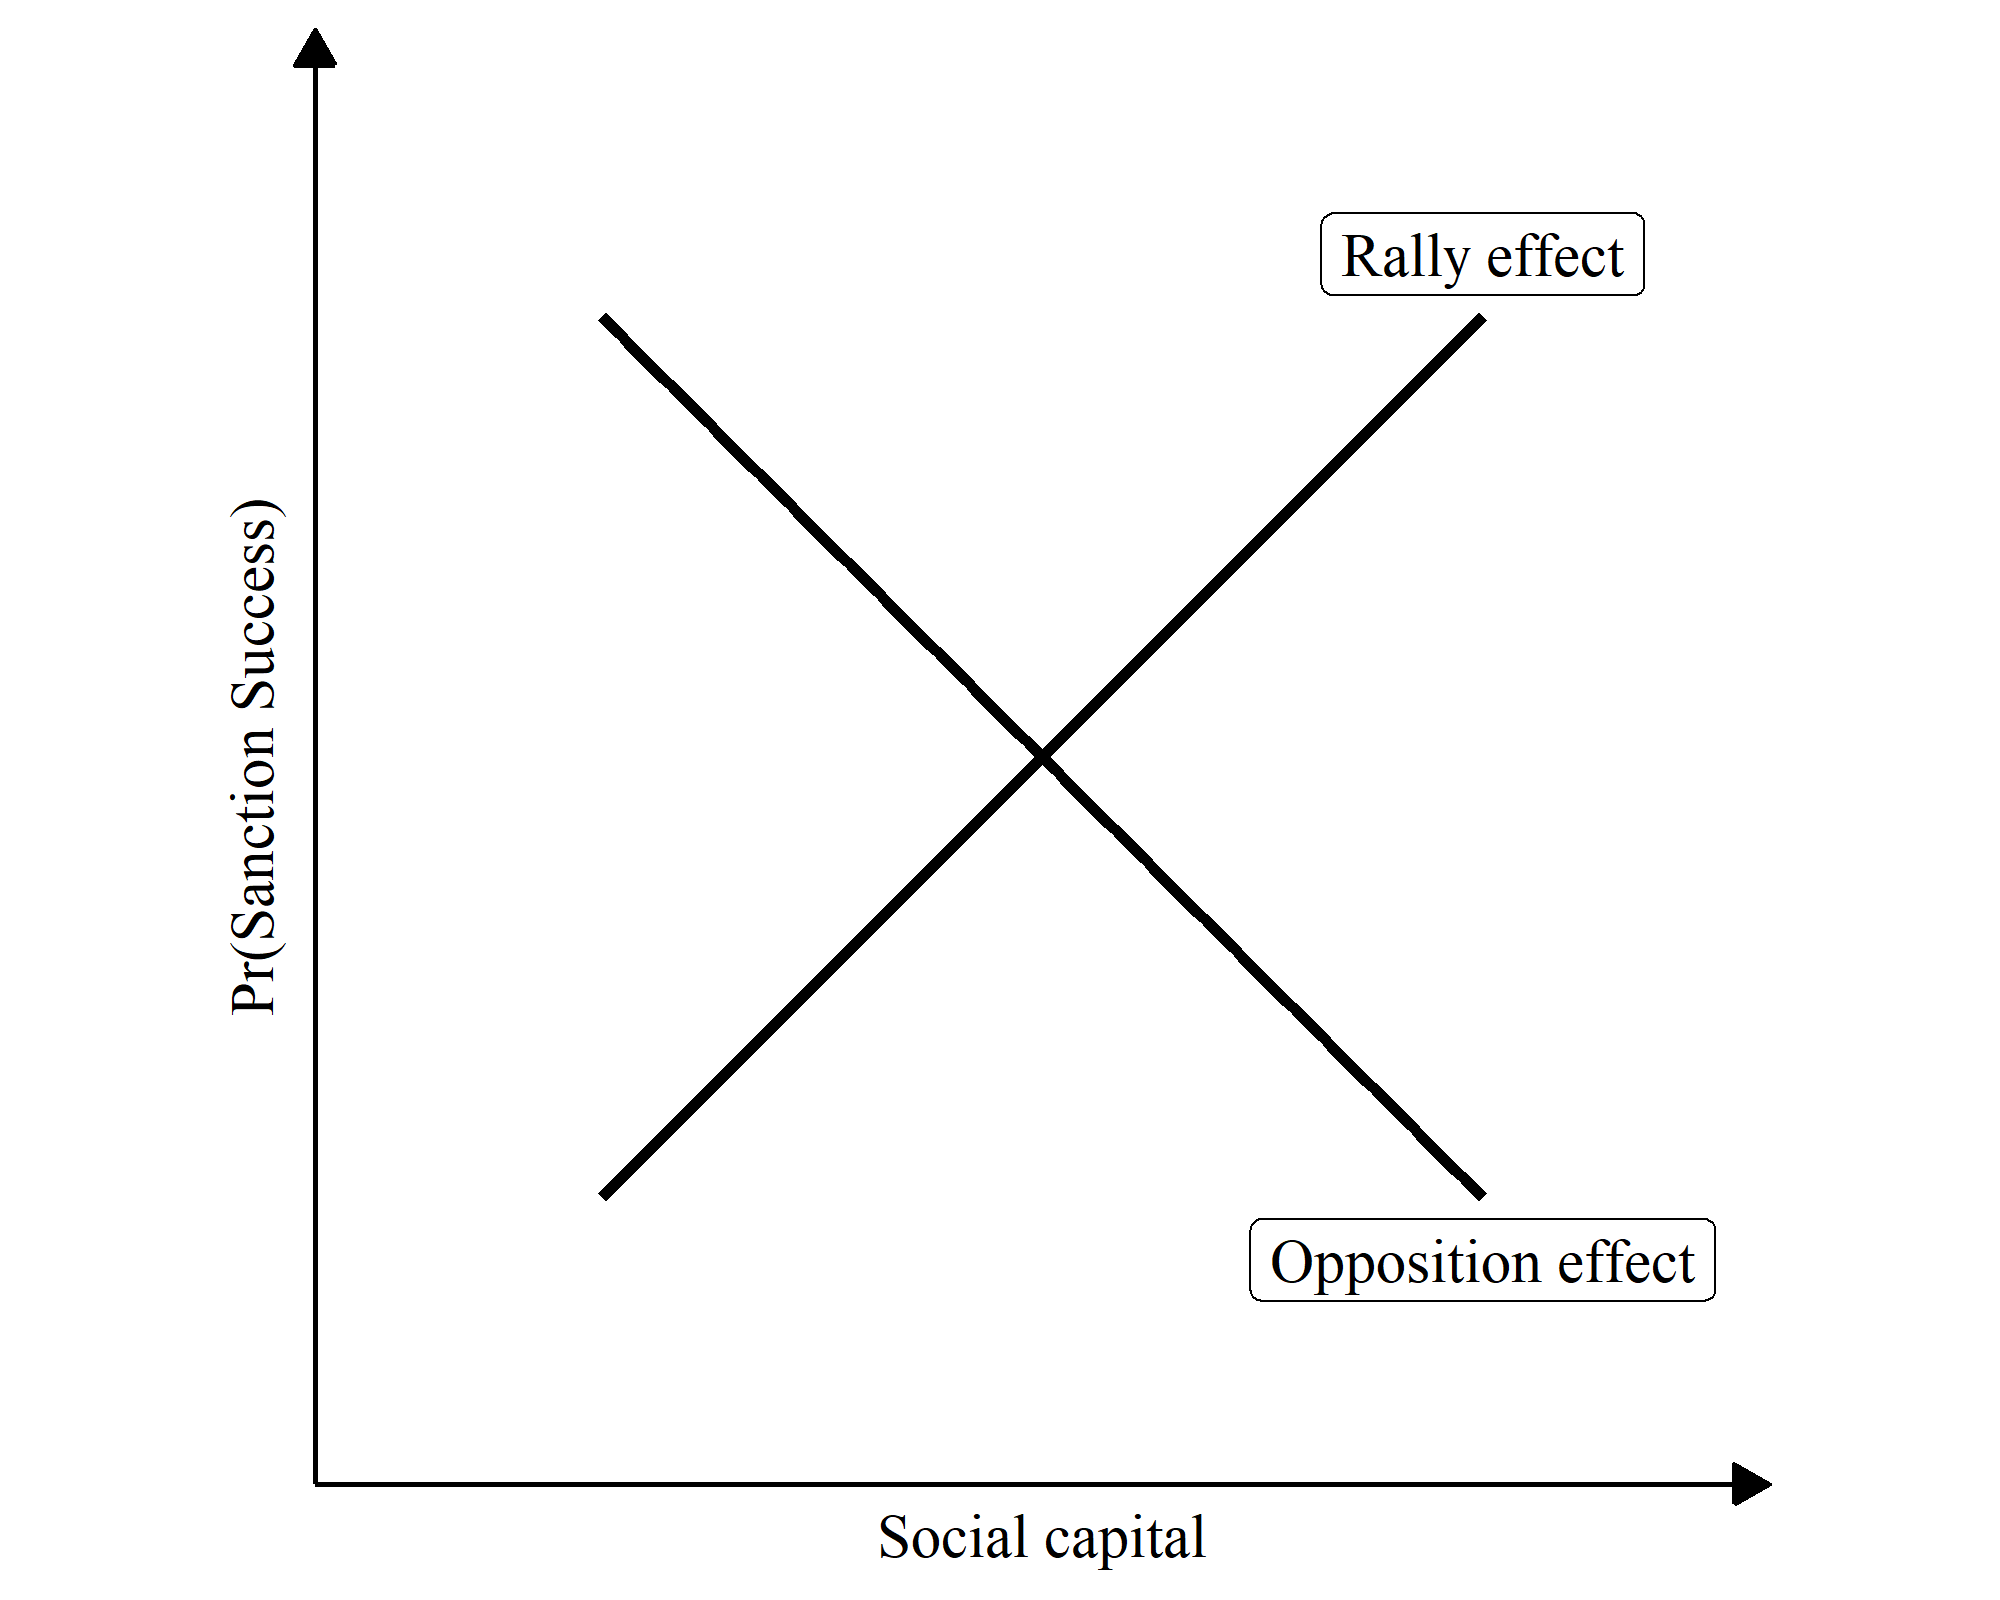
\includegraphics[width=0.65\linewidth]{figures/equilibrium} 

}

\caption{\label{fig1} Offsetting effects of social capital on the likelihood sanctions are successful.}\label{fig:unnamed-chunk-1}
\end{figure}

Figure \ref{fig1} summarizes the theoretical expectations based on the
conflicting \emph{opposition effect} and \emph{rally effect} of social
capital. The success of sanctions depends on the degree of social
capital in the sanctioned country. Social capital helps reveal citizen
preferences effectively through collective action, which can function
negatively as a veto constraint (\emph{opposition effect}) or positively
as defenders of the sanctioned country's leader (\emph{rally effect}).
The question now shifts to determining which effect is greater. As the
degree of social capital increases, will the afflicted populace
mobilize, oppose the leader's policy, and display the \emph{opposition
effect}? Or will the populace support its leader in defying sanctions
through the \emph{rally effect}? It is unclear which effect prevails as
social capital increases. In this study, we posit that both effects are
theoretically plausible, and that empirical evidence will reveal which
outweighs the other.

\hypertarget{data-variables-and-methods}{%
\section{Data, Variables, and
Methods}\label{data-variables-and-methods}}

\hypertarget{data}{%
\subsection{Data}\label{data}}

In this study, we subject the theory of social capital, information, and
sanctions to empirical tests using three datasets. One is the Threat and
Imposition of Sanctions (TIES) project (Version 4.0), which covers
imposition of sanctions from 1945 to 2005 \citep{morgan2009a}, and the
other is the dataset from the World Values Survey (WVS). Combining these
datasets, the individual instances of sanctions across 1981--2005 are
analyzed. WVS has conducted one of the largest cross-national opinion
surveys since 1981 regularly, and we utilize the data from the survey to
operationalize social capital by measuring survey questions related to
trust, membership, and confidence. We include Countries in all six waves
of the WVS. Wave 1 covers 1981--1984, Wave 2 covers 1990--1994, Wave 3
covers 1995--1998, Wave 4 covers 1999--2004, Wave 5 covers 2005--2009,
and Wave 6 covers 2010--2014. Although Wave 1 posed survey questions
about trust, membership, and confidence to only nine countries, the
number rose to 17 in Wave 2, 53 in Wave 3, 40 in Wave 4, 57 in Wave 5,
and 59 in Wave 6.\footnote{The Appendix lists countries that
  participated in the survey.}

\hypertarget{variables}{%
\subsection{Variables}\label{variables}}

Our dependent variable identifies the success of sanctions as a binary
variable using the variable, \emph{Final Outcome}, from the TIES data.
Sanctions have been defined as successful and are assigned a value of 1
if the termination of the sanctions leads to `Partial Acquiescence by
the Target State', `Total Acquiescence by Target State', and `Negotiated
Settlement'. The other outcomes such as `Capitulation by the sender',
and `Stalemate', are coded as failed outcomes and are assigned a value
of 0.\footnote{Since we assume sanctions are already in place, we
  exclude outcomes that end at the threat stage.}

Our main explanatory variables in this study, are the average of each
country's degree of social capital, which is operationalized through one
question concerning trust, two concerning membership, and four
concerning confidence from all six waves of WVS. Using the online
analysis, we merge the averages of responses per wave by country,
combining all questions on trust, membership, and confidence using their
mean scores. For example, if 38.4\% of survey respondents answered,
`Most people can be trusted', we coded it as 38.4\% of people who
maintain feelings of general trust. Details for each question per
category are presented below.

All waves pose the same question for trust and confidence. The principal
question concerning general trust include the following: \emph{Generally
speaking, would you say that most people can be trusted or that you need
to be very careful in dealing with people?} The responses include,
`\emph{Most people can be trusted}', `\emph{Can't be too careful}', and
`\emph{No answer}'.

Membership is separated into two questions. Waves 1, 3, and 5 use one
set of formatted question and waves 2 and 4 use another. Waves 1, 3, and
5 ask the following questions: \emph{Please look carefully at the
following list of voluntary organizations and activities and select
which, if any, do you belong to.} Waves 2 and 4 ask: \emph{Now I am
going to read out a list of voluntary organizations; for each one, could
you tell me whether you are a member, an active member, or not a member
of that type of organization?} The first membership question has three
answer choices (\emph{active member, inactive member, and not a
member}). Questions for Waves 2 and 4 offer two options (\emph{belongs,
do not belong}). We use both questions to observe survey membership in
political parties and professional associations. Because the number of
answer choices for each question differs, we combine the active and
inactive membership from the first set of questions to maintain
consistency.

Confidence entails one question in all waves: \emph{I am going to name
numerous organizations. For each one, could you tell me how much
confidence you have in them: is it a great deal of confidence, quite a
lot of confidence, not very much confidence, or none at all?} We measure
confidence in political parties, government, parliament, and the justice
system.

As control variables, we include political (\emph{Alliance} and
\emph{Target democracy}), economic (\emph{Target ln(GDPPC)}), issue
(\emph{Issue salience}), and geographical variables (\emph{Contiguity}
and \emph{Distance}). \emph{Alliance} uses the Correlates of War Formal
Alliance dataset \citep{gibler2009a}. If the sanctioned country is not
allied with the sanctioning country, the variable is coded 0.
\emph{Target Democracy} measures the degree of democracy in the
sanctioned country based on the V-Dem project's Electoral democracy
index. It measures how much the ideal of electoral democracy is achieved
in a given year and given country. The variable varies from 0 (least
democratic) to 1 (most democratic) based on the concept of
\emph{Polyarchy} \citep{coppedge2020a}. \emph{Target GDP per capita} is
the logged GDP per capita of the sanctioned country, which measures its
economic power. \emph{Issue salience} identifies the leading
institutions in the country that initiates sanctions. They include
bureaucracy, legislature, executive or government, judiciary, and
others. We expect the salience of the issue at stake to increase when
legislative or executive branches, rather than a bureaucracy or
judiciary, initiates sanctions. Elected politicians have incentives to
publicize opponents' positions and their own. Thus, \emph{Issue
salience} equals 1 if \emph{Sanction Identity} in the TIES dataset
indicates legislature, executive, or government and 0 otherwise.
\emph{Distance} measures the physical distance between the sanctioning
and sanctioned countries to control for geographical proximity, as
neighboring countries can be more exposed to sanctions than remote
countries. We use the logged values of \emph{Distance.}
\emph{Contiguity} is a six-category variable that measures the
contiguity between the sanctioning and sanctioned countries. The
Appendix summarizes statistics for all variables.

\hypertarget{methods}{%
\subsection{Methods}\label{methods}}

Because the dependent variable is binary, we use probit analysis with
robust standard errors to evaluate the hypotheses. When data are
time-series cross-sectional data with repeated observations on units
\citep{stimson1985a}, the dependent variable are likely to be not
independently and identically distributed \citep{King2001a, Zorn2006a}.
We estimate the robust standard errors to correct variance-covariance
estimates addressing potential heteroscedasticity. Our results report
the statistical significance at the level of 10\%, 5\%, and 1\% to
address potential issues driven by the small number of observations. We
also estimate the predicted probabilities of successful sanctions as a
function of a series of explanatory variables to show the substantial
implications of the results.

\hypertarget{results}{%
\section{Results}\label{results}}

\begin{longtable}[]{@{}lccc@{}}
\caption{\label{tab1} Effet of social capital (\emph{Trust} and
\emph{Memberships}) on success of sanctions}\tabularnewline
\toprule
& Model 1 & Model 2 & Model 3\tabularnewline
\midrule
\endfirsthead
\toprule
& Model 1 & Model 2 & Model 3\tabularnewline
\midrule
\endhead
Trust & -0.023 (0.013)+ & &\tabularnewline
Membership: Political Party & & -0.027 (0.029) &\tabularnewline
Membership: Prof.Association & & & -0.034 (0.033)\tabularnewline
Contig & -2.689 (1.566)+ & -1.647 (2.122) & -1.586
(2.117)\tabularnewline
Distance & 1.546 (0.911)+ & 0.905 (1.243) & 0.881 (1.238)\tabularnewline
lnGDPpc & -0.071 (0.363) & 0.453 (0.414) & 0.434 (0.430)\tabularnewline
Salience & 0.885 (0.455)+ & 1.319 (0.514)* & 1.385
(0.547)*\tabularnewline
Alliance & 0.767 (0.424)+ & 0.205 (0.588) & 0.444 (0.525)\tabularnewline
Target Democracy & -1.328 (1.042) & -1.315 (1.025) & -1.237
(1.007)\tabularnewline
Num.Obs. & 116 & 94 & 94\tabularnewline
AIC & 115.0 & 87.3 & 87.3\tabularnewline
BIC & 137.1 & 107.6 & 107.6\tabularnewline
Log.Lik. & -49.521 & -35.633 & -35.632\tabularnewline
\bottomrule
\end{longtable}

\textbf{Note:} \^{}\^{} + p \textless{} 0.1, * p \textless{} 0.05, ** p
\textless{} 0.01

Table \ref{tab1}. reports the regression results when using \emph{Trust}
(Model 1.), \emph{Membership: Political party} (Model 2.), and
\emph{Membership: Prof.~association} (Model 3.) as the main explanatory
variables for social capital. All three models indicate that
coefficients for the main explanatory variables are negative and
significant at 5\% in Models 1. and 2. and at 10\% for Model 3. This
finding implies that as trust, membership in political parties, and
political associations in the sanctioned country increase--i.e., as the
degree of social capital increases in the sanctioned country--the
likelihood that sanctions are successful declines significantly.

It is evident from Table \ref{tab1} that the \emph{rally effect} is more
prominent than the \emph{opposition effect}. The sanctioned populace is
more likely to support its leader in defying sanctions. There is no
evidence whether or how intensively the leader of the sanctioned country
is involved in persuading the populace to rally support, however, we do
know that the \emph{opposition effect} is not functioning as might be
expected. It seems that, on average, social capital prompts the
sanctioned populace to sympathize with its leader's defiance of
sanctions rather than regarding them as an unnecessary tariff to be
abolished. Thus, it would be poor counsel to advise strengthening or
expanding sanctions to incite the populace to unite against its leader
for concessions. Such counsel ignores that the \emph{rally effect}
dominates the \emph{opposition effect} in the sanctioned country.

\begin{figure}

{\centering 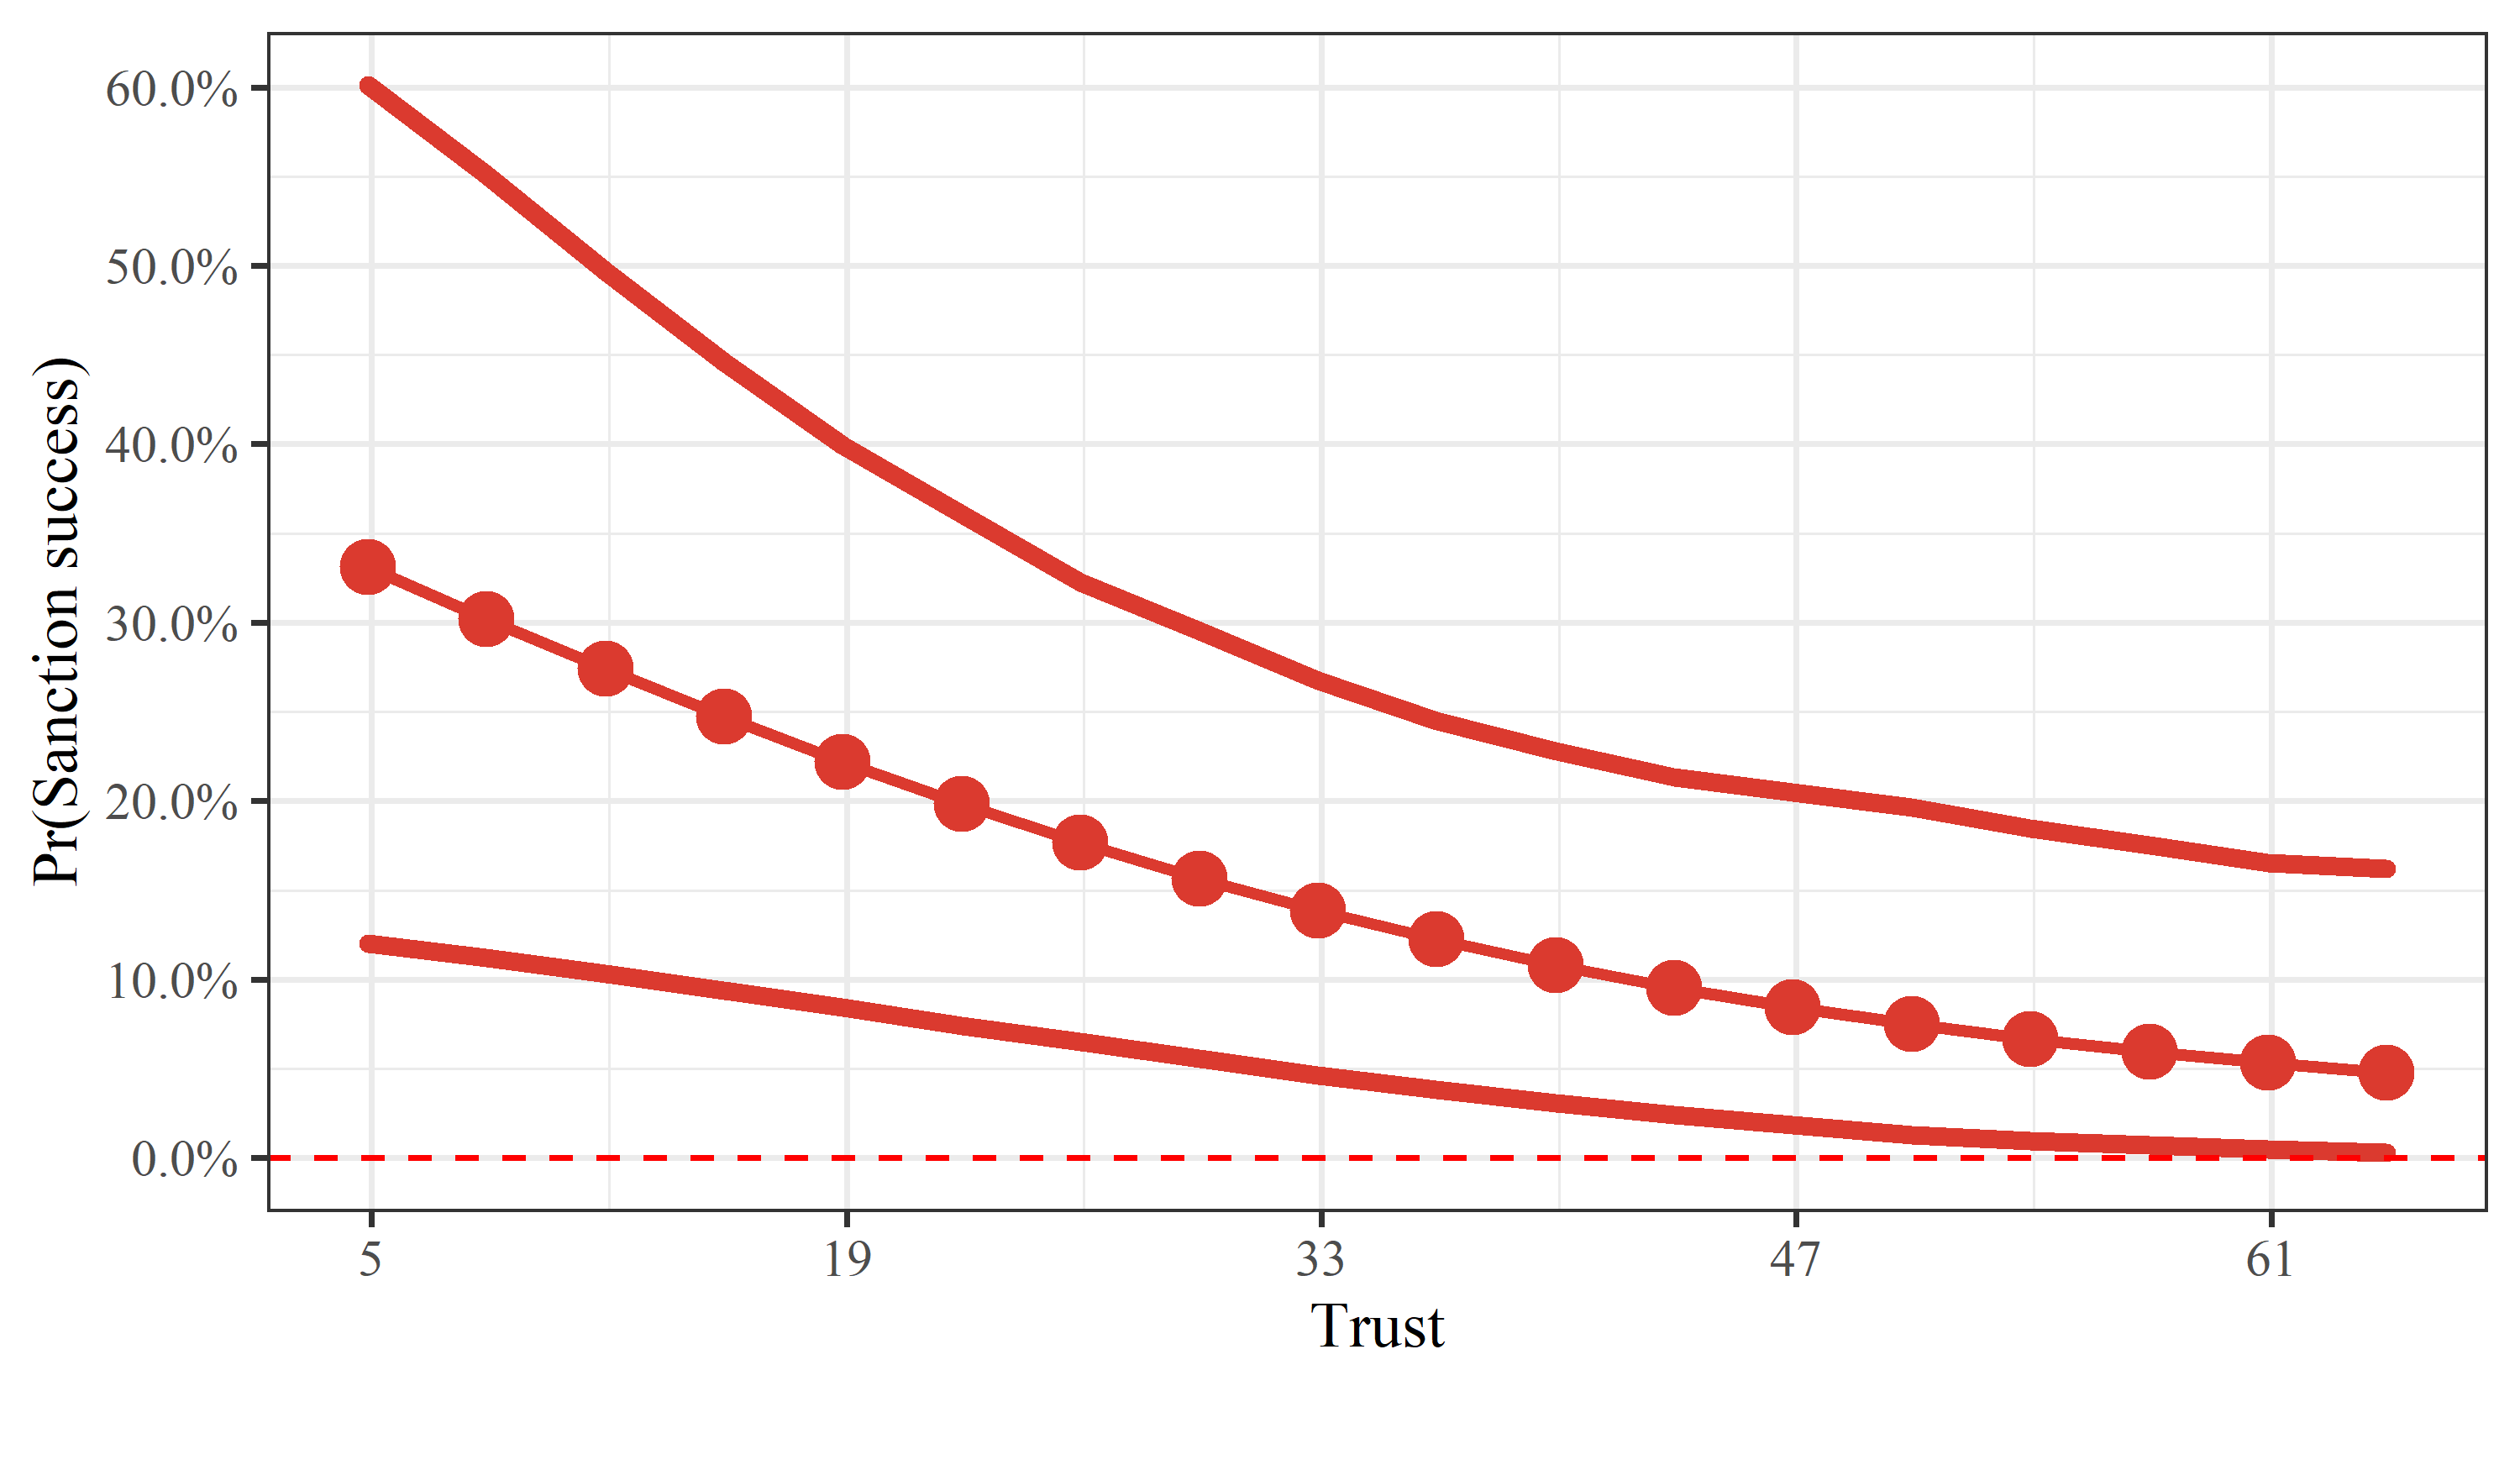
\includegraphics[width=0.65\linewidth]{figures/figure2} 

}

\caption{\label{fig2} Predicted probability of successful sanctions as a function of \textit{Trust}.}\label{fig:unnamed-chunk-3}
\end{figure}
\begin{figure}

{\centering 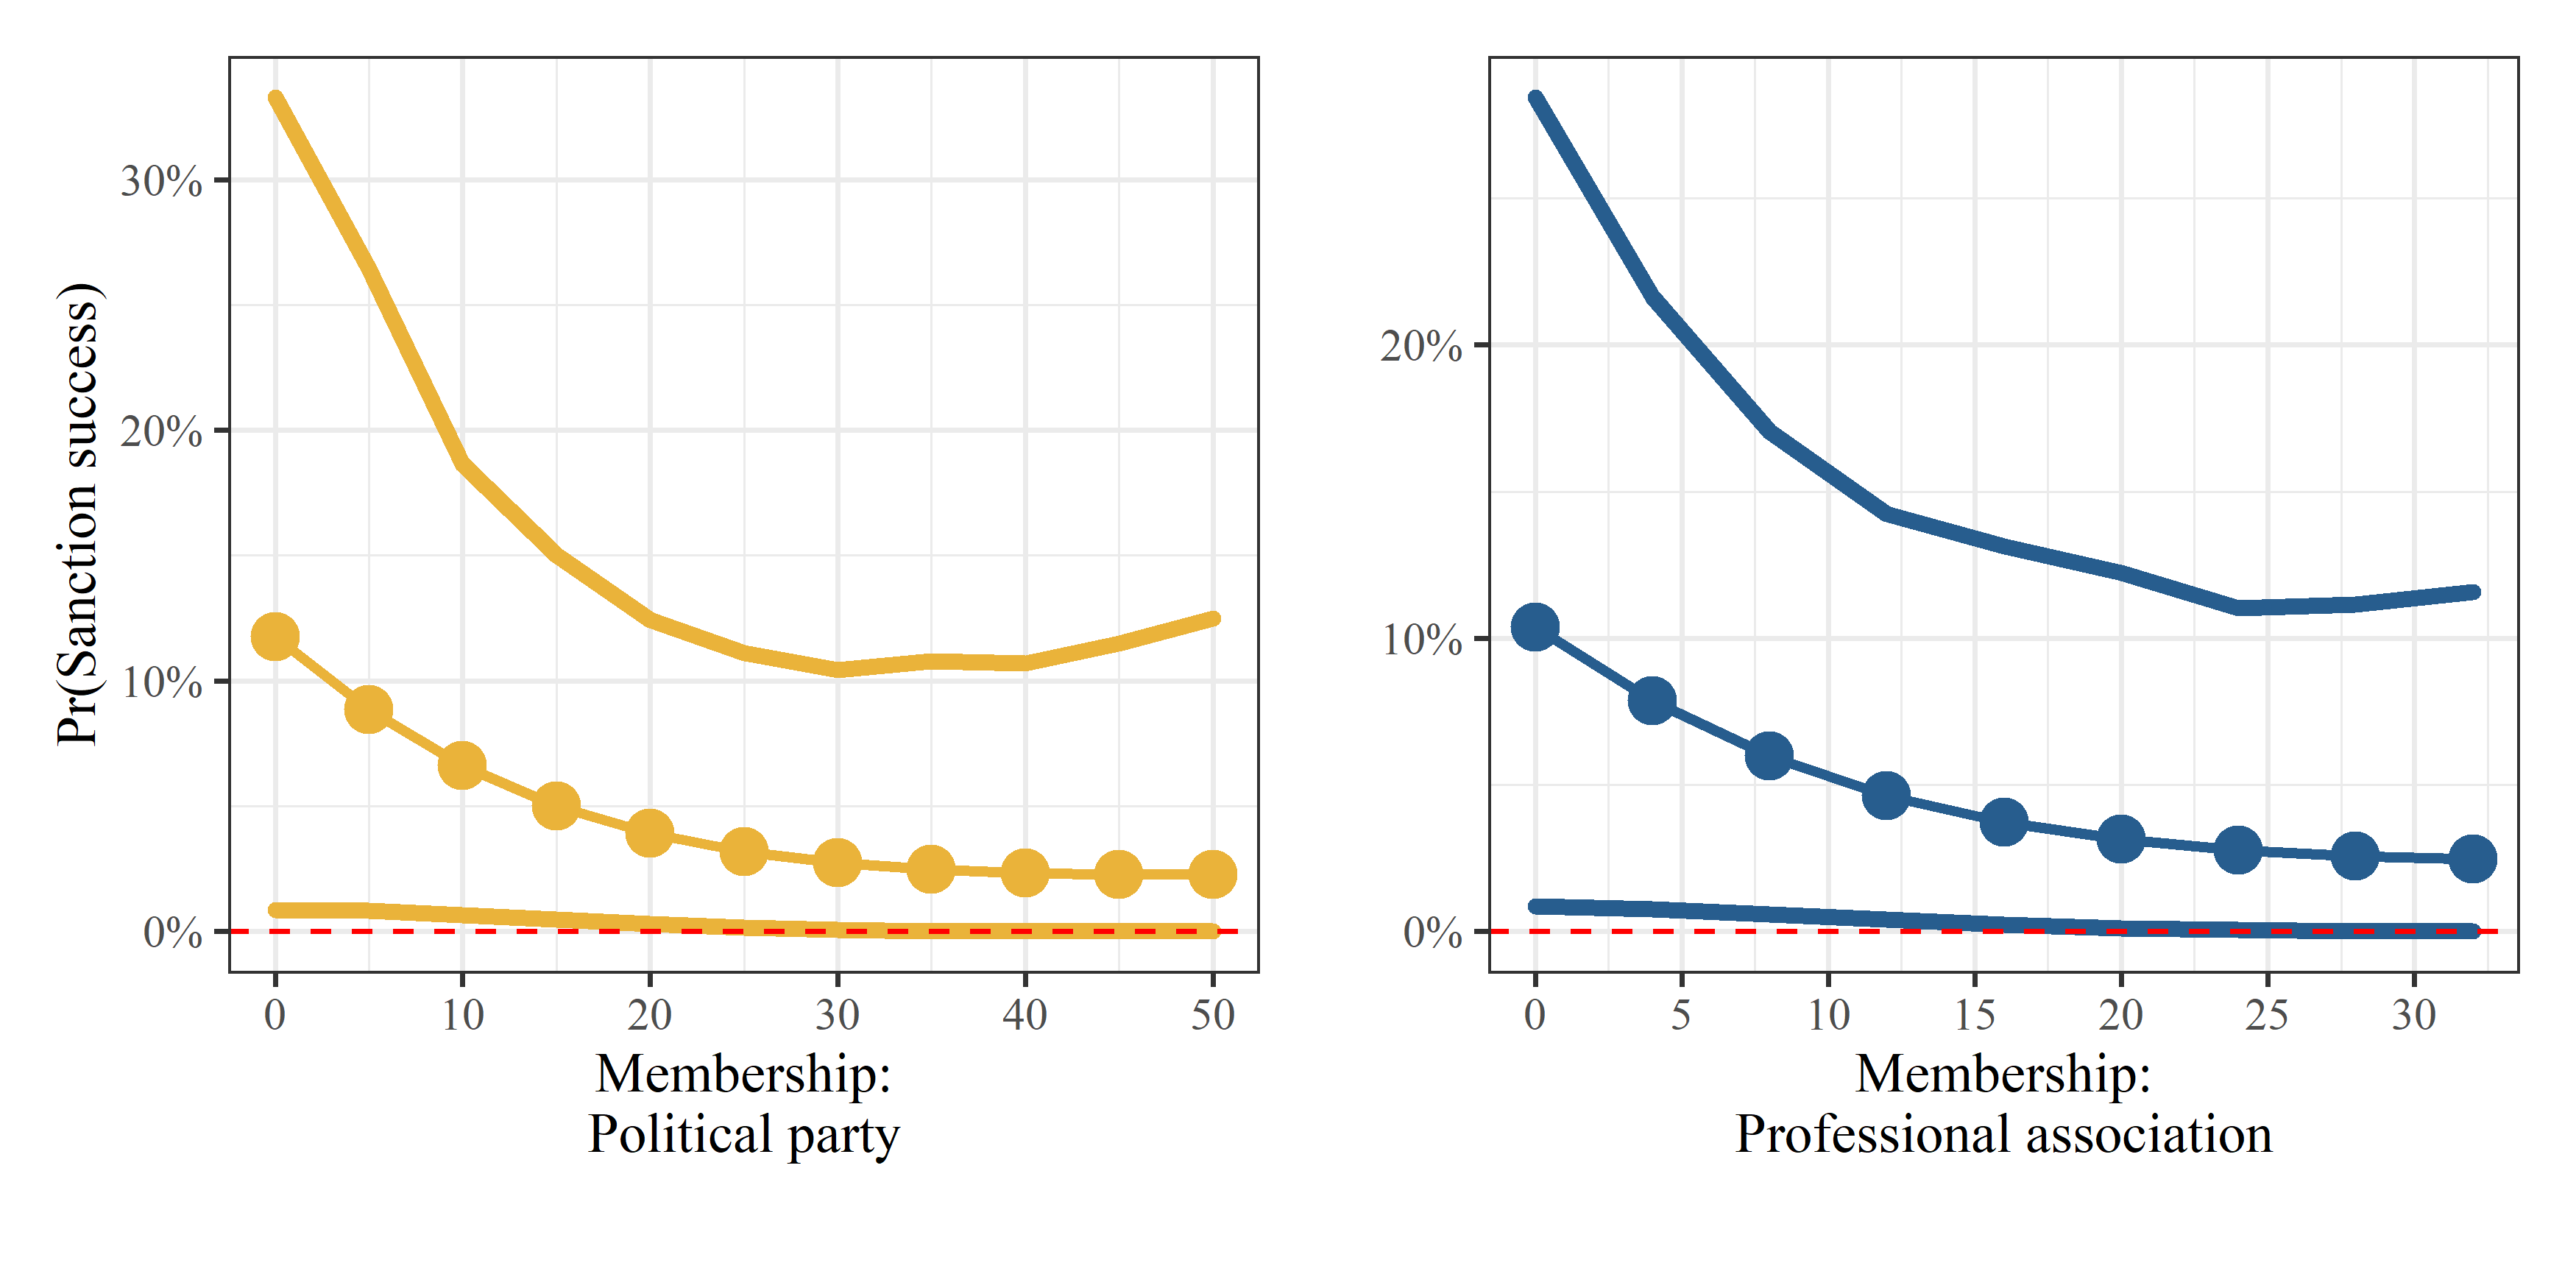
\includegraphics[width=0.65\linewidth]{figures/figure3} 

}

\caption{\label{fig3} Predicted probability of successful sanctions as a function of Membership: \textit{Political party} and \textit{Professional association}.}\label{fig:unnamed-chunk-4}
\end{figure}

Figures \ref{fig2} and \ref{fig3} display predicted probabilities of
successful sanctions as a function of the three social capital measures
while setting all other variables to their means: \emph{Trust} (Figure
\ref{fig2}), \emph{Membership: Political Party}, and \emph{Membership:
Professional Association} (Figure \ref{fig3}). The figures partially
confirm the \emph{Rally Effect Hypothesis}: successful sanctions are
less likely as social capital increases with respect to Trust. Trust
reduces the success rate of sanctions by more than 30\% when we use the
variable using its lowest and highest values.

Although two membership variables are not statistically significant,
their patterns are similar: membership in political parties and
associations reduce the likelihood that sanctions will succeed by about
10\% and 7\%, respectively. This finding implies that the populace tends
to blame the sanctioning country and, more important, this tendency
becomes more prominent as the capacity for mobilization increases.

Table \ref{tab2} displays estimation results for the success of
sanctions after using confidence variables in WVS to measure social
capital. We use Confidence in \emph{Political Party} (Model 1),
\emph{Government} (Model 2), \emph{Parliament} (Model 3), and
\emph{Courts} (Model 4.), and ask how the confidence of the sanctioned
populace in key institutions affects the likelihood that the leader of
the sanctioned country resists sanctions. Although the findings are not
statistically significant, their patterns with respect to the effects of
social capital on the sanction's success endorse those in Table
\ref{tab1}. As confidence in political institutions increases in the
sanctioned country, its leader appears less likely to make concessions,
reducing the likelihood that sanctions succeed on average.

\begin{table}
\caption{\label{tab2} Efffet of social capital (*Confidence)* on success of sanctions}
\centering
\resizebox{\columnwidth}{!}{%
\begin{tabular}[t]{lcccc}
\toprule
  & Model 1 & Model 2 & Model 3 & Model 4\\
\midrule
Confidence: Political party & -0.018 (0.052) &  &  & \\
Confidence: Government &  & -0.015 (0.031) &  & \\
Confidence: Parliament &  &  & -0.021 (0.034) & \\
Confidence: Courts &  &  &  & -0.034 (0.028)\\
Contig & -2.456 (1.521) & -2.297 (1.432) & -2.603 (1.597) & -0.571 (2.539)\\
Distance & 1.434 (0.886) & 1.365 (0.828)+ & 1.526 (0.938) & 0.297 (1.495)\\
lnGDPpc & -0.144 (0.433) & -0.150 (0.392) & -0.223 (0.439) & -0.511 (0.737)\\
Salience & 0.323 (0.522) & 0.577 (0.654) & 0.637 (0.439) & 1.093 (0.638)+\\
Alliance & 0.830 (0.581) & 0.785 (0.524) & 0.877 (0.522)+ & 0.803 (0.786)\\
Target Democracy & -1.431 (1.428) & -2.732 (1.628)+ & -1.753 (1.368) & -0.685 (1.552)\\
\midrule
Num.Obs. & 76 & 68 & 102 & 65\\
AIC & 89.3 & 80.9 & 112.3 & 74.0\\
BIC & 108.0 & 98.7 & 133.3 & 91.4\\
Log.Lik. & -36.656 & -32.456 & -48.149 & -29.009\\
\bottomrule
\multicolumn{5}{l}{\textsuperscript{} + p $<$ 0.1, * p $<$ 0.05, ** p $<$ 0.01}\\
\end{tabular}%
}
\end{table}

Combined with results of Table \ref{tab1}, social capital measured by
dimensions of trust, membership, and confidence point in favor of the
\emph{rally effect}. Even though the sanctioned populace must suffer
economic hardship, people seem willing to defend their leader.

\begin{figure}[ht]

{\centering 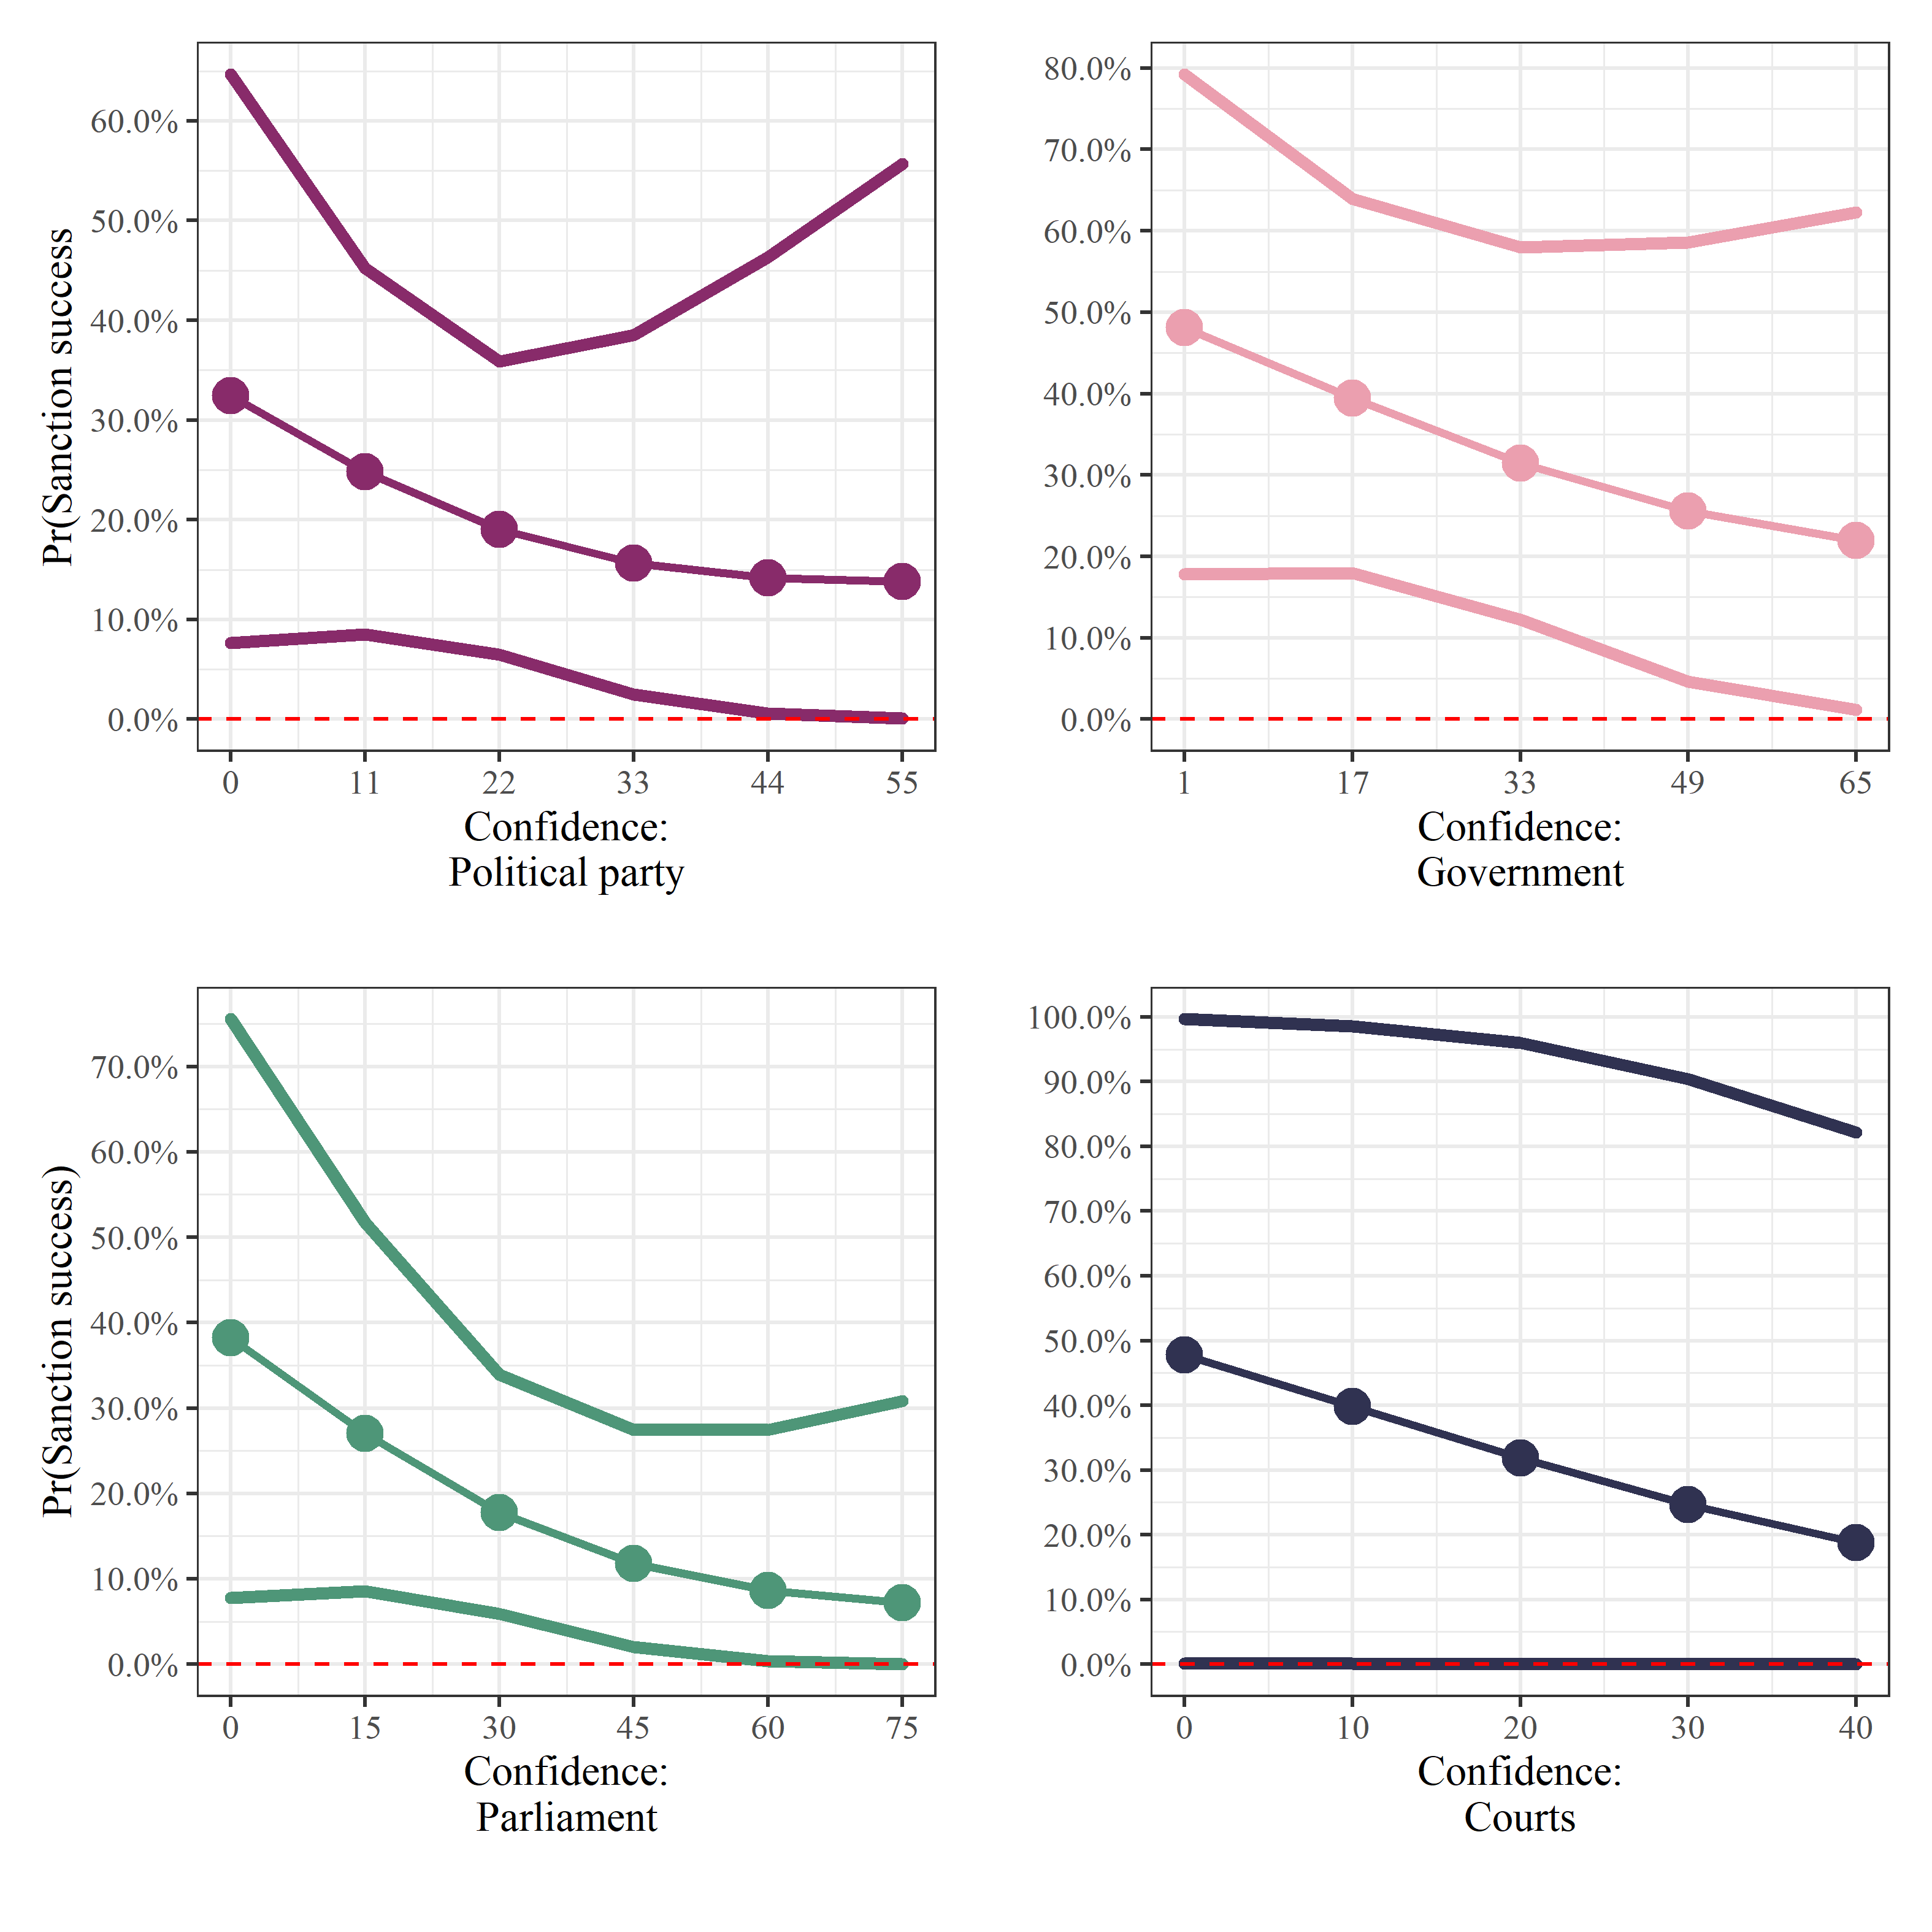
\includegraphics[width=0.65\linewidth]{figures/figure4} 

}

\caption{\label{fig4} Predicted probability of successful sanctions as a function of Confidence: \textit{Political party, government, parliaments}, and \textit{courts}.}\label{fig:unnamed-chunk-6}
\end{figure}

Figure \ref{fig4} displays the substantive effects of confidence
variables on the predicted probability of sanctions being successful.
Each subfigure reveals that when we vary the confidence variables from
their minimum to maximum values, the predicted probability of successful
sanctions drops by about 17\% to 26\% on average. Although the
confidence variables do not reveal statistical significance, their
patterns convey that it is more likely to support the \emph{Rally Effect
Hypothesis} over the \emph{Opposition Effect Hypothesis}.

In sum, we provide a micro-foundation for the rally-round-the-flag
effect. When the sanctioned country has internal cohesion through trust,
membership in political parties or associations, and confidence in
institutions, the sanctioned populace generally supports its leader.
Social capital is useful for the leader of the sanctioned country to
fight sanctions. The likelihood of successful sanctions is more likely
to diminish as a result.

\hypertarget{discussion}{%
\section{Discussion}\label{discussion}}

Our results imply that high social capital can support the target
government and deter the success of sanctions. WVS data provides no
information about North Korea, however, numerous sources indicate that
job losses are the major negative effect of sanctions affecting North
Korea's populace. UN Resolution 2270 on 2 March 2016 was reinforced by
closing the Kaesong industrial complex, which left 50,000 North Koreans
unemployed and deprived North Korea of \$100 million annually.

Furthermore, UN Resolution 2375 passed on 11 September 2017 also
prohibited a substantial part of North Korea's imports and exports, as
well as joint ventures and labor exports with Russia and China,
increasing the number of jobless people. Despite these harsh conditions,
there was no collective opposition from citizens within North Korea.
Scholars often assume social capital does not exist in North Korea
because the government is notoriously repressive. However, interviews
with North Korean refugees reveal that trust and community bonds exist,
however, they are not maintained from the bottom up as is more typical
of social capital in democratic countries.

According to refugees, the most feared organization in North Korea is
the State Security Department (SSD), which functions as the secret
police, operating concentration camps, and monitoring and identifying
`defectors' who express dissatisfaction with the regime every day. This
itself imposes a social network, contriving social capital, creating
communities that spy on families and exiling people who oppose
government policies to prevent the dispersion of ideas (Mazarr, 2007;
Scobell, 2005). With the use of the `Weekly Life Review Session', the
SSD was able to further control the society by making people monitor and
alert each other. Although known as the `Weekly Life Review Session',
there is an accurate descriptive translation that is more recognized,
which is `Self-Criticism and Mutual-Criticism Session'
\citep{lankov2013a}.

Furthermore, this type of control was also present in the media. Like
Russia's Pravda, or China's \emph{Renimn RiBao}, North Korea has the
\emph{Rodong Shinmun} editorial which plays a crucial role in
effectively spreading and engraving North Korean regime's messages to
its citizens by introducing and reinforcing the messages of Kim Jong-un
and the Workers' Party of Korea \citep{ford2018a}.

In addition, as it is already well known, North Korea's citizens have
high levels of pride for living according to the spirit of `Juche' which
enables good socio-structural conditions for collectivism to develop.
The agricultural production has a fundamental trait in North Korea's
social capital as it operates through cooperative farms and collective
activities from various organizations under the Worker's Party. As such,
Kim Jong-un and the other politicians create a controlled \emph{rally
effect} by forcefully creating and imposing social capital that supports
them.

North Korea's political elite dominates the allocation of resources and
flow of information in nearly all segments of society. Reports from the
SSD, however, reveals strong community bonds and support for government.
These feelings may be imposed exogenously, as people know that the SSD
monitors them, however, they are confirmed by refugees who insist that
trust and community bonds persist. Moreover, the government has
manipulated the populace into believing it is victimized by
international forces. This enhances trust and community bonds and raises
popular support for the country's policies. The populace suffers under
sanctions, losing work and income, paying inflating prices because
imports are limited, and being deprived of aid, however, networks of
associations within the community sustain rather than oppose the regime.
Thus, social capital is engineered to support the regime and to create
opposition toward sanctions. Because social capital is extensively
manipulated, sanctions have been unsuccessful, and the rally effect
operates in North Korea.

As an illustration of its effectiveness, in June 2016 the North Korean
government initiated a 200-day mass mobilization following a similar
70-day mobilization in May. Both propaganda-driven events began after
the UN strengthened its sanctions following North Korea's 2016 nuclear
test. Originally intended to kick off a new five-year economic plan, the
mobilization encouraged North Koreans to remain opposed to sanctions and
to support the regime. Although North Koreans are more or less obligated
to participate, the campaign's leaders encourage and praise ordinary
people to instill national pride and to urge them to persevere despite
strengthened sanctions. These mass mobilizations generate support for
the government and social capital-building nationalism.

\hypertarget{conclusion}{%
\section{Conclusion}\label{conclusion}}

This empirical study has illustrated that the influence of social
capital can exert two unifying but contradictory effects on the success
of economic sanctions. The \emph{opposition effect} posits that
sanctions are likely to be more successful as social capital increases,
whereas the \emph{rally effect} contends that sanctions are less likely
to be successful as social capital increases. In this study, we
investigated these effects using data from the WVS to measure trust,
membership, and confidence as the main independent variable of social
capital and TIES for the dependent variable of successful sanctions.
After adding control variables and evaluating hypotheses using probit
analysis with robust standard errors, we found that the empirical data
supports the \emph{Rally Effect Hypothesis} over the \emph{Opposition
Effect Hypothesis}. As the degree of social capital increases in a
sanctioned country, the likelihood of successful sanctions declines
significantly. Our findings imply that comprehensive sanctions aimed at
the populace will not engender immediate opposition against its leader,
as conventional wisdom suggests. The \emph{rally effect} can present an
additional impediment to be considered when designing sanctions.

Although insightful, finding correlations and imputing causality between
social capital and sanctions is a new field that lacks the benefit of
prior research. The operationalization of social capital may be open to
empirical disagreements as we incorporate the new facet of confidence.
However, our measurements can be justified under the notion that the
forms of confidence we include are the captured feelings about both the
government and the society that are factors in understanding social
capital.

Although insightful, finding correlations and imputing causality between
social capital and sanctions is a new field that lacks the benefit of
prior research. The operationalization of social capital may be open to
empirical disagreements as we incorporate the new facet of confidence.
However, our measurements can be justified under the notion that the
forms of confidence we include capture feelings about both government
and society that are factors in understanding social capital.

\newpage





\newpage
\singlespacing 
\bibliography{r-references.bib}

\end{document}
